%------------------------------------------------------------------------------
% Author(s):
% Varaun Ramgoolie
%
% Copyright:
%  Copyright (C) 2020 Brad Bachu, Arjun Mohammed, Varaun Ramgoolie, Nicholas Sammy
%
%  This file is part of Applied-Mathematics-Unit2 and is distributed under the
%  terms of the MIT License. See the LICENSE file for details.
%
%  Description:
%     Year: 2006 C
%     Module: 3
%     Question: 5
%------------------------------------------------------------------------------

%------------------------------------------------------------------------------
% 5 a
%------------------------------------------------------------------------------

\begin{subquestions}
	
\subquestion

We are given two masses which are connected by a string over a smooth, weightless pulley.

\begin{subsubquestions}
	
	\subsubquestion
	
	\textbf{\textit{Sketch and Translate:}} \\ \\
	\begin{figure}[H]
		\begin{center}
			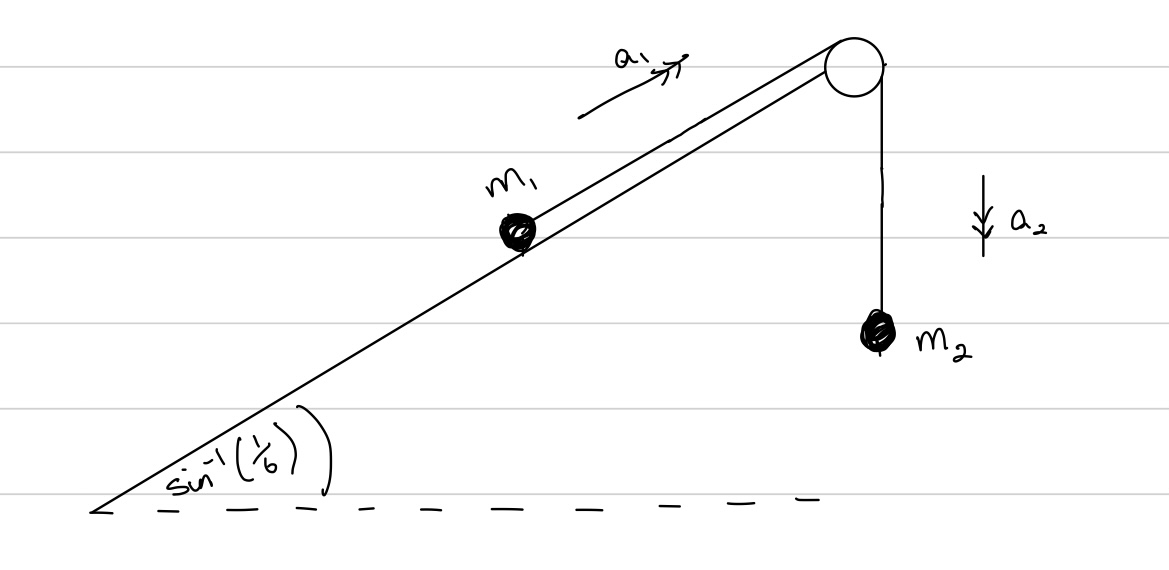
\includegraphics[scale=0.25]{../2006/figures/2006q5-1}
			\caption{\label{2006:q5:Sketch1} Pulley System.}
		\end{center}
	\end{figure}	
	We are asked to find the acceleration of the system given. This problem is a pulley problem together with an inclined plane situation and so, we should think about what we know about tension and forces in the context of masses connected by the string.
	
	
	
	
	\textbf{\textit{Simplify and Diagram:}} \\ \\
	\begin{figure}[H]
		\begin{center}
			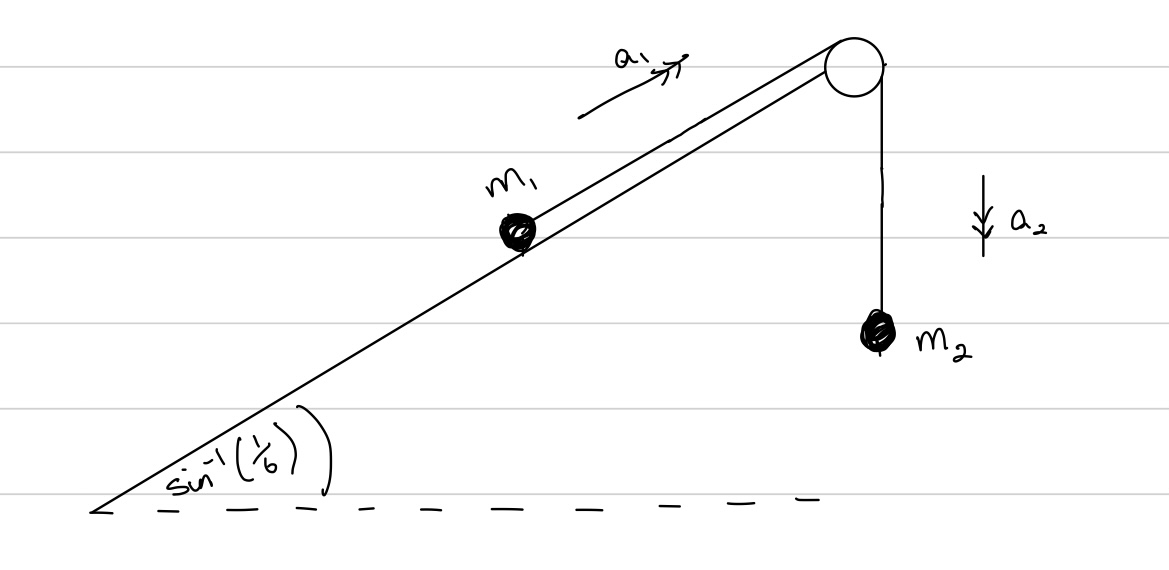
\includegraphics[scale=0.25]{../2006/figures/2006q5-1}
			\caption{\label{2006:q5:Diagram1} All forces on Pulley System.}
		\end{center}
	\end{figure}
	We will assume that both bodies behave as point particles. We will also assume that the mass of the string is 0 and inextensible. Thus, we know that the speed (and the magnitude of the acceleration) of both particles must be the same. Since the pulley is smooth, no energy is lost to friction. We should consider how the forces act on the different weights and motivate our solution from there. We will define the following:
	\begin{itemize}
		\item $\vec{W_1}$ is the weight of the 12kg mass,
		\item $\vec{W_2}$ is the weight of the 8kg mass,
		\item $\vec{T_1}$ is the tension on the string from the 12kg mass to the pulley,
		\item $\vec{T_2}$ is the tension on the string from the 8kg mass to the pulley,
		\item $\vec{R}$ is the normal reaction force of the 12kg mass,
		\item $m_1$ is the mass of the 12kg mass, $m_1=12$,
		\item $m_2$ is the mass of the 8kg mass, $m_1=8$.
	\end{itemize}
	We will find the Resultant Force in the direction of the acceleration of both the masses and use Newton's Second Law to solve for the acceleration. We will assume that there is no acceleration perpendicular to the plane.
	
	
	\textbf{\textit{Represent Mathematically:}} \\ \\ 
	Let us denote the displacements of the 12kg and 8kg masses as $y_1$ and $y_2$ respectively. As the string is inextensible, we know that,
	\begin{align}
		|y_1| & = |y_2| \nn \\
		\implies \ddd{y_1}{t} & = \ddd{y_2}{t} \nn \\
		\implies \ddd{^2y_1}{t^2} & = \ddd{^2y_2}{t^2} \nn \\
		a_1 & = a_2 = a \,.
	\end{align}
	where $a_1$ and $a_2$ are the acceleration of the 12kg and 8kg mass respectively.
	
	From the assumption that the string is massless, we also get that,
	\begin{equation}
		|T_1| = |T_2| = T \,.
	\end{equation}
	
	We will resolve $W_1$ in terms of the unit vectors parallel ($\xhat$) and perpendicular ($\yhat$) to the plane as,
	\begin{equation}
		\vec{W_1} = -\sin\left(\arcsin\left(\frac{1}{6}\right)\right)|W_1|\xhat - \cos\left(\arcsin\left(\frac{1}{6}\right)\right)|W_1|\yhat \,.
	\end{equation}
	
	Let us first consider the forces on the 12kg mass. From Newton's 2nd Law in the direction of the acceleration (the $\xhat$ direction), we get that,
	\begin{align}
		\sum F & = m_1a_1 \nn \\
		T_1 -\sin\left(\arcsin\left(\frac{1}{6}\right)\right)|W_1| & = m_1a_1 \label{2006:q5:SimEqn1} \,.
	\end{align}
	
	Let us then consider the forces on the 8kg mass. From Newton's 2nd Law, we get that,
	\begin{align}
		\sum F & = m_2a_2 \nn \\
		m_2g-T_2 & = m_2a_2 \label{2006:q5:SimEqn2} \,.
	\end{align}
	
	
	
	
	\textbf{\textit{Solve and Evaluate:}} \\ \\
	By substituting our values, we can see that \reqs{2006:q5:SimEqn1}{2006:q5:SimEqn2} become,
	\begin{align}
		T_1 -\frac{1}{6}m_1g & = m_1a_1 \nn \\
		\implies T - 2g & = 12a \label{2006:q5:SimEqn3} \\
		& \text{and} \nn \\
		m_2g-T_2 & = m_2a_2 \nn \\
		\implies 8g-T & = 8a \label{2006:q5:SimEqn4} \,.
	\end{align}
	
	Solving \reqs{2006:q5:SimEqn3}{2006:q5:SimEqn4} simultaneously, we get,
	\begin{align}
		(\text{\req{2006:q5:SimEqn3}+\req{2006:q5:SimEqn4}}): (T-2g)+[8g-T] & = (12a)+[8a] \nn \\
		6g & = 20a \nn \\
		\implies a & = 2.94ms^{-2}\,.
	\end{align} 
	
	%------------------------------------------------------------------------------
	
	\subsubquestion
	
	\textbf{\textit{Solve and Evaluate:}} \\ \\
	Substituting our value of $a$ into \req{2006:q5:SimEqn3}, we get that,
	\begin{align}
		T & = 12(2.94) + 2g \nn \\
		  & = 54.88N \,.
	\end{align}
	
	%------------------------------------------------------------------------------
	
	\subsubquestion
	
	\textbf{\textit{Simplify and Diagram:}} \\ \\
	As we have assumed that there is no acceleration perpendicular to the plane (and by extension, no resultant force), we can use Newton's Second Law on the 12kg mass and solve for $\vec{R}$.
	
	
	
	
	\textbf{\textit{Represent Mathematically:}} \\ \\
	By resolving $\vec{R}$, we get that,
	\begin{equation}
		\vec{R} = |\vec{R}|\yhat \,.
	\end{equation}  
	
	Considering  $\yhat$ components of the forces on the 12kg mass and applying Newton's Second Law, we get that,
	\begin{align}
		\sum F = |\vec{R}|-\cos\left(\arcsin\left(\frac{1}{6}\right)\right)|\vec{W_1}| = 0 \label{2006:q5:REqn1}\,.
	\end{align}
	
	
	
	
	\textbf{\textit{Solve and Evaluate:}} \\ \\
	From \req{2006:q5:REqn1}, we get that,
	\begin{align}
		|\vec{R}| & = \cos\left(\arcsin\left(\frac{1}{6}\right)\right)12g \nn \\
		          & = \frac{\sqrt{35}}{6}\times 12g \nn \\
		          & = 19.6\sqrt{35} = 115.96N \,. 
	\end{align}
	
\end{subsubquestions}	
	
%------------------------------------------------------------------------------
% 5 b
%------------------------------------------------------------------------------
	
\subquestion

\textbf{\textit{Sketch and Translate:}} \\ \\
\begin{figure}[H]
	\begin{center}
		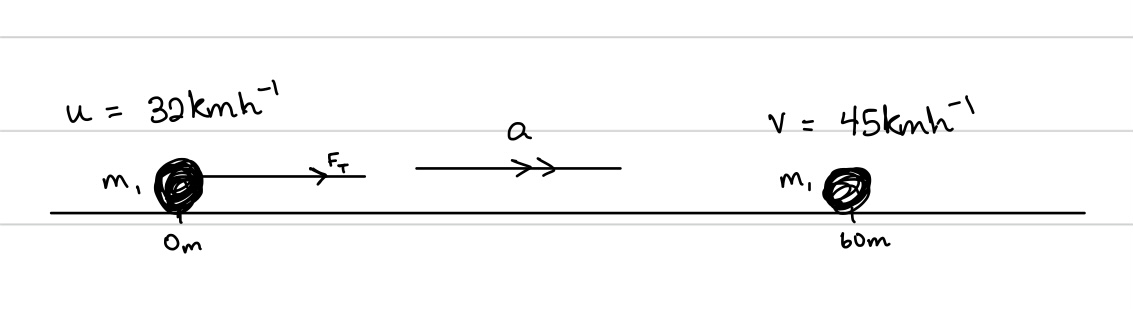
\includegraphics[scale=0.25]{../2006/figures/2006q5-2}
		\caption{\label{2006:q5:Sketch2} Movement of car.}
	\end{center}
\end{figure}	
To find the tractive force of the car, we will need to use our equations of motion and Newton's Second Law.




\textbf{\textit{Simplify and Diagram:}} \\ \\
\begin{figure}[H]
	\begin{center}
		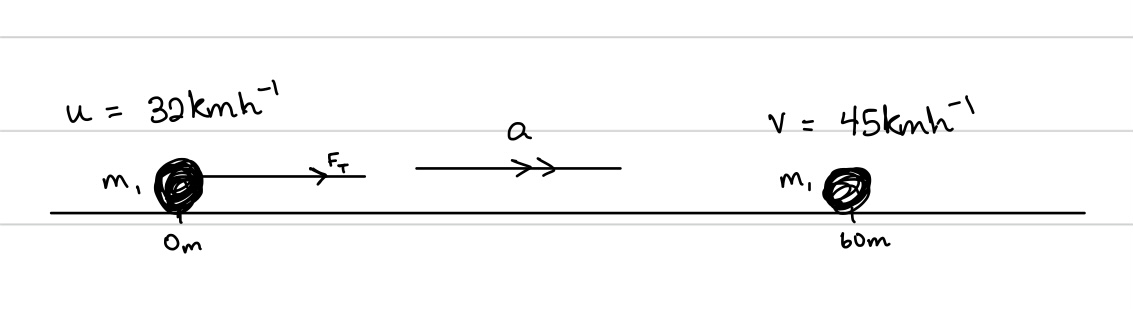
\includegraphics[scale=0.25]{../2006/figures/2006q5-2}
		\caption{\label{2006:q5:Diagram2} Movement of car.}
	\end{center}
\end{figure}
We will assume that the car accelerates with constant velocity. We will define the following:
\begin{itemize}
	\item $u$ is the initial velocity of the car, $u=\frac{80}{9}ms^{-1}$,
	\item $v$ is the final velocity of the car, $v=\frac{25}{2}ms^{-1}$,
	\item $s$ is the distance traveled by the car, $s=60m$,
	\item $a$ is the acceleration of the car,
	\item $m$ is the mass of the car, $m=1250kg$,
	\item $F_T$ s the tractive force of the car.
\end{itemize}
To find the tractive force, we will find the acceleration of the car, use $F_T$ as the resultant force on the car, and apply Newton's Second Law.
	

	
	
\textbf{\textit{Represent Mathematically:}} \\ \\
To find $a$, we will use,
\begin{equation}
	v^2=u^2+2as \label{2006:q5:AEqn1} \,.
\end{equation}

From Newton's Second Law, we get that,
\begin{equation}
	F_T = ma \label{2006:q5:FEqn1} \,.
\end{equation}




\textbf{\textit{Solve and Evaluate:}} \\ \\
Using \req{2006:q5:AEqn1}, we get that,
\begin{align}
	\left(\frac{25}{2}\right)^2 & = \left(\frac{80}{9}\right)^2 + 120a \nn \\
	\implies a & = \frac{\left(\frac{25}{2}\right)^2-\left(\frac{80}{9}\right)^2}{120} \nn \\
	           & = 0.644ms^{-2} \,.
\end{align}

Using \req{2006:q5:FEqn1}, we get that,
\begin{align}
	F_T & = 1250 \times 0.644 \nn \\
	    & = 805N \,.
\end{align}

\end{subquestions}